\documentclass{article}
\usepackage[utf8]{inputenc}
\usepackage{amsmath}
\usepackage{amssymb}
\usepackage{booktabs}
\usepackage{cancel}
\usepackage{enumitem}
\usepackage{graphicx}
\usepackage{mathtools}
\usepackage{mdframed}
\usepackage{multirow}
\usepackage{pgfgantt}
\usepackage{pdflscape}
\usepackage{bbm}
\usepackage[margin=1in]{geometry}
\usepackage{biblatex} 
\addbibresource{library.bib}

\title{NE8 Lecture 4: the discrete ordinates/S$_N$ method}
\author{Paul Cosgrove and Zi Liang Tan}
\date{September 2022}

\begin{document}

\maketitle

Previously we developed two common methods applied in numerically solving the transport equation in the context of lattice physics: the collision probability method (CPM) and the method of characteristics (MoC). Here we develop one other very common method known as either the discrete ordinates method or the S$_N$ method (where S stands for angular \textit{Segments} and $N$ is the order of the quadrature set applied). It has many similarities with MoC but differs in some key respects which will be discussed.

Much of the presentation of this lecture follows \cite{Hebert}.

\section{The discrete ordinates approximation}

In deriving MoC the `discrete ordinates approximation' was briefly discussed. This essentially means discretising $\mathbf{\Omega}$, the angular variable of the transport equation. As a result, we only consider the transport equation along some set $\{\mathbf{\Omega}_n\}$ of angles such that we are now solving $N$ equations of the form:
\begin{equation}\label{eq:transport_DO}
    \begin{split}
 \mathbf{\Omega}_n\cdot\nabla\psi_n + \Sigma_\mathrm{tr}\psi_n
    =\frac{1}{4\pi}\frac{\bar{\nu}\Sigma_\mathrm{f}}{ k_\mathrm{eff}}\phi + \frac{1}{4\pi}\Sigma_\mathrm{s}\phi\;\mathrm{,}
    \end{split}
\end{equation}
where $\mathbf{\Omega}_n$ is one of the chosen angles and $\psi_n =\psi(\mathbf{\Omega}_n)$. In discretising angles, we still must be able to approximate integrals over angle, e.g., to estimate the scalar flux. This can be done by associating with each $\mathbf{\Omega}_n$ a corresponding angular weight, $w_n$, normalised such that:
\begin{equation}\label{eq:quad}
	\int_{4\pi}\mathrm{d}\Omega = \sum_{n=1}^{N}w_n = 4\pi\;\mathrm{.}
\end{equation}
As such, the scalar flux can be approximated as:
\begin{equation}
	\phi\approx\sum^N_{n=1}\psi_n w_n\;\mathrm{.}
\end{equation}
Obviously, the accuracy of the approximation improves as $N$ increases, but this implies having to solve more equations and expend more computational effort.

\subsection{Numerical integration and the importance of quadrature choice}

To get a feel for how important choosing a good quadrature is, here is an example problem. Say we have a function:
\begin{equation}
	f(\mu) = \sinh(\mu)\left[1+\sin(2\pi \mu)\right]\;\mathrm{.}
\end{equation}
In the domain of $\mu=-1$ to $\mu=1$, this function has the analytic integral:
\begin{equation}
	I = \int^1_{-1}\mathrm{d}\mu\;\sinh(\mu)\left[1+\sin(2\pi \mu)\right] = -\frac{4\pi \sinh(1)}{1+4\pi^2}\approx -0.364836735717049\;\mathrm{.}
\end{equation}
Suppose that we aren't very good at analytic integrals and wanted to calculate this numerically. Recall that the integral $I$ of $f(\mu)$ can be interpreted as the area under its curve -- one straightforward method will be to approximate this area by rectangles whose areas are easy to calculate. Suppose we divide the domain $(-1,1)$ into $N$ intervals of width $\Delta \mu = 2/N$ and we use each interval to construct rectangles of width $\Delta \mu$ and height $f(\mu_n)$ where $\mu_n$ is the midpoint of each interval. Then the integral $I$ is approximated as the total area of these rectangles as:
\begin{equation}\label{SN3}
	I = \int^1_{-1}\mathrm{d}\mu\;f(\mu)\approx \sum^N_{n=1}\Delta \mu f(\mu_n)\;\mathrm{.}
\end{equation}
Figure \ref{fig1} gives an example of a ten-rectangle approximation $f_{10}(\mu)$ to the function $f(\mu)$.
\begin{figure}[h!]
	\centering
	\begin{minipage}{0.5\textwidth}
		\centering
		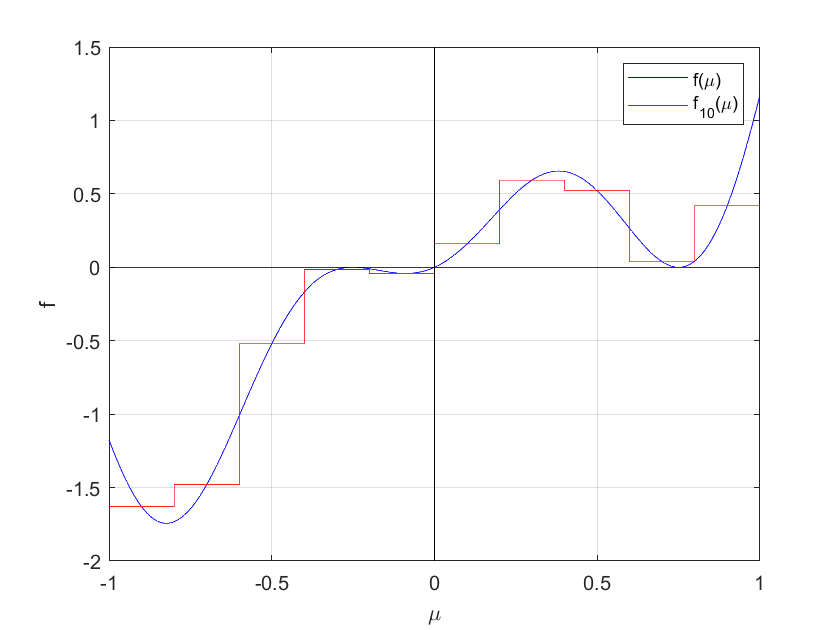
\includegraphics[width=1\textwidth]{images/fig1.png}
		\caption{Ten-rectangle approximation $f_{10}(\mu)$ of $f(\mu)$.}
		\label{fig1}
	\end{minipage}\hfill
	\begin{minipage}{0.5\textwidth}
		\centering
		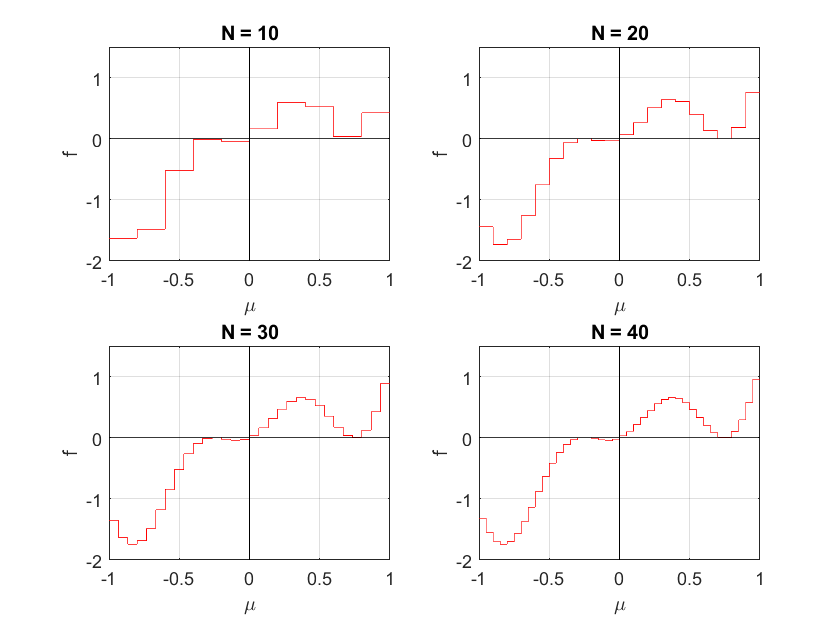
\includegraphics[width=1\textwidth]{images/fig2.png}
		\caption{$N$-rectangle approximations of $f(\mu)$.}
		\label{fig2}
	\end{minipage}
\end{figure}
We expect the $N$-rectangle approximation to improve with increasing $N$ as the shape of $f(\mu)$ is better captured (see Fig.~\ref{fig2}). For each $N$-rectangle approximation we calculate its area and calculate its relative error with respect to the exact value of $I$ in Fig.~\ref{fig3}. We see that the absolute relative error indeed decreases with increasing $N$, reflecting the better approximation with increasing $N$.
\begin{figure}[h!]
	\centering
	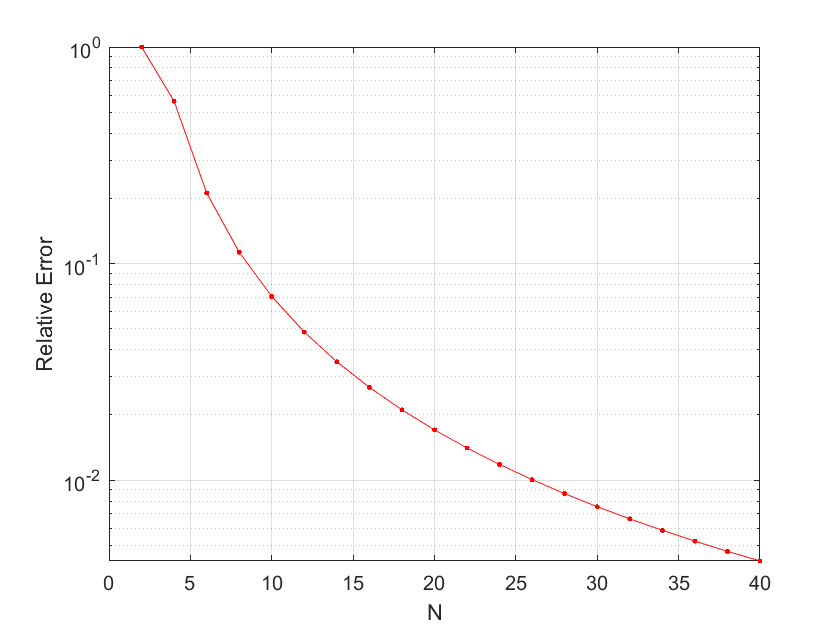
\includegraphics[width=0.6\linewidth]{images/fig3.png}
	\caption{Absolute relative error of integrated $N$-rectangle approximations of $f(\mu)$.}
	\label{fig3}
\end{figure}

The $N$-rectangle approximation is nice, but we would like to do better. Taking inspiration from Eq.~\eqref{SN3}, we would like to seek approximations of the form:
\begin{equation}\label{eq:integral}
	I=\int_{-1}^1\,f(\mu)\,d\mu\approx\sum_{n=1}^N w_n\,f(\mu_n)
\end{equation}
The idea is thus: for some well-chosen value of $\mu_n$ (which is called the \textit{abscissa}), we evaluate the function value $f(\mu_n)$ and multiply it with a well-chosen factor $w_n$ (which is called the \textit{weight}) that indicates the contribution of this function value to the integral. The sum of these weighted quantities makes up the approximated integral value.

A `well-chosen' quadrature set of abscissa and weights $\{\mu_n,w_n\}$ should be such that we can achieve smaller approximation errors with fewer calculations of $f$ (put alternatively, with smaller $N$). This is generally dependent on the specific features of the considered problem, and therefore `well-chosen' quadrature sets are usually problem-dependent.

For our problem in this note, we will adopt the \textit{Gauss-Legendre quadrature set}. Fig.~\ref{fig4} gives a table of Gauss-Legendre quadrature sets for $N=2,4,6,8,10,12$. Note first that every $\mu_n$ abscissa reported has a corresponding $-\mu_n$ abscissa with the same weight $w_n$. Second, if we're in slab geometry, these weights don't sum to $4\pi$ as in Eq.~\eqref{eq:quad}, but instead sum to 2 (because the domain is that in Eq.~\eqref{eq:integral}) -- if we had a 3D quadrature set then it would indeed sum to $4\pi$. 

Fig.~\ref{fig5} shows a comparison of the absolute relative errors in approximating $I$ via the Gauss-Legendre and rectangle approximations. We see that using the Gauss-Legendre quadrature set achieves smaller approximation errors at smaller $N$. One of the other convenient features of the Gauss-Legendre quadrature is that the set of order $N$ can exactly integrate Legendre polynomials up to the same order (hence the name), which helps mitigate errors in transport solutions with anisotropic scattering.
\begin{figure}[h!]
    \centering
    \begin{minipage}{0.45\textwidth}
        \centering
        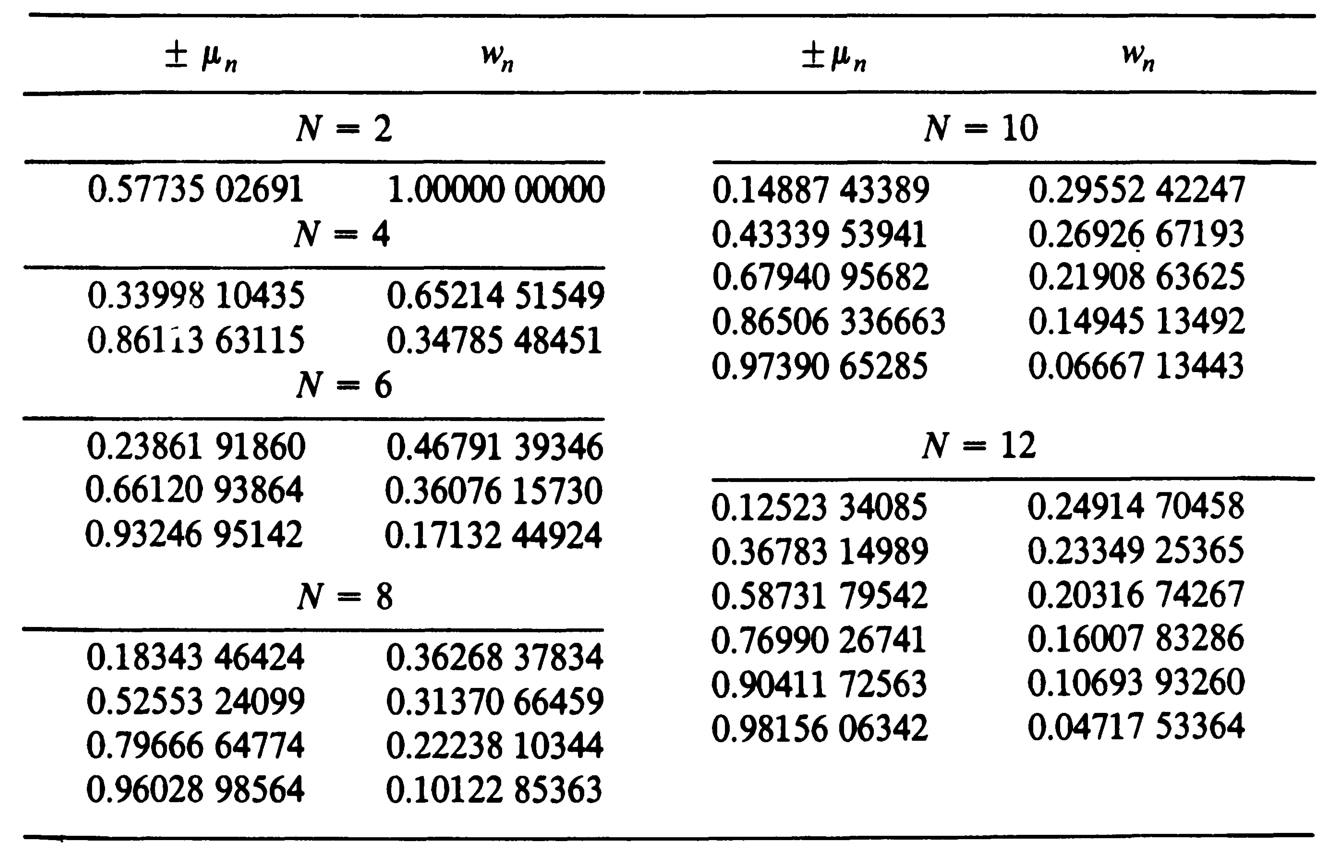
\includegraphics[width=1\textwidth]{images/fig4.png}
        \caption{Table of Gauss-Legendre quadrature \\ sets~\cite{Lewis}}
        \label{fig4}
    \end{minipage}\hfill
    \begin{minipage}{0.5\textwidth}
        \centering
        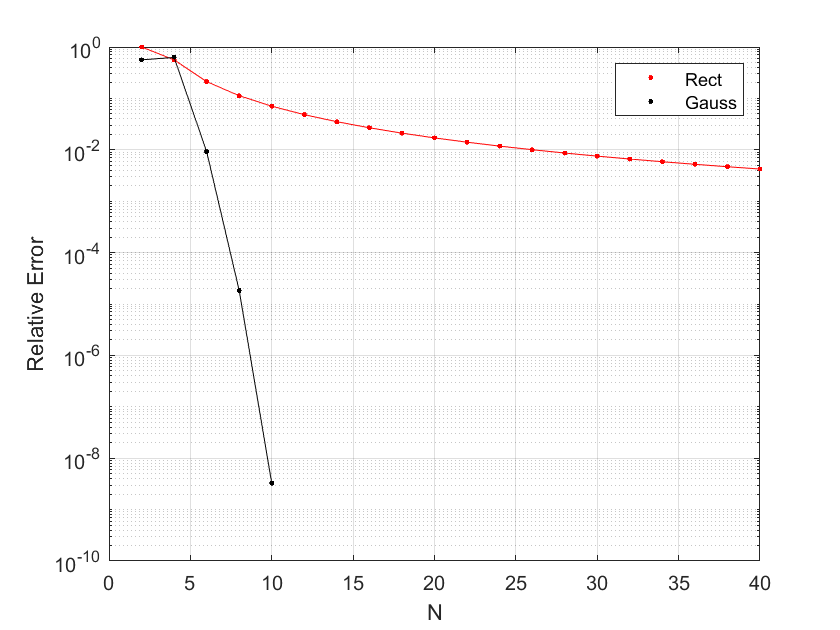
\includegraphics[width=1\textwidth]{images/fig5.png}
        \caption{Absolute relative error of Gauss- \\ Legendre versus rectangle approximation.}
        \label{fig5}
    \end{minipage}
\end{figure}

Many other choices of quadrature exist, although one nearly universal feature is choosing a set which is \textbf{octant symmetric on the unit sphere} because problems often do not have a favoured direction; as such, quadrature sets often can be visualised as in Fig.~\ref{fig:3D_quad}. We also tend to choose $N$ as an even number to ensure we do not have any angles pointing directly towards the poles of the unit sphere -- these can cause numerical difficulties, e.g., divisions by 0 or ambiguities in handling boundary conditions.

\begin{figure}[h!]
	\centering
	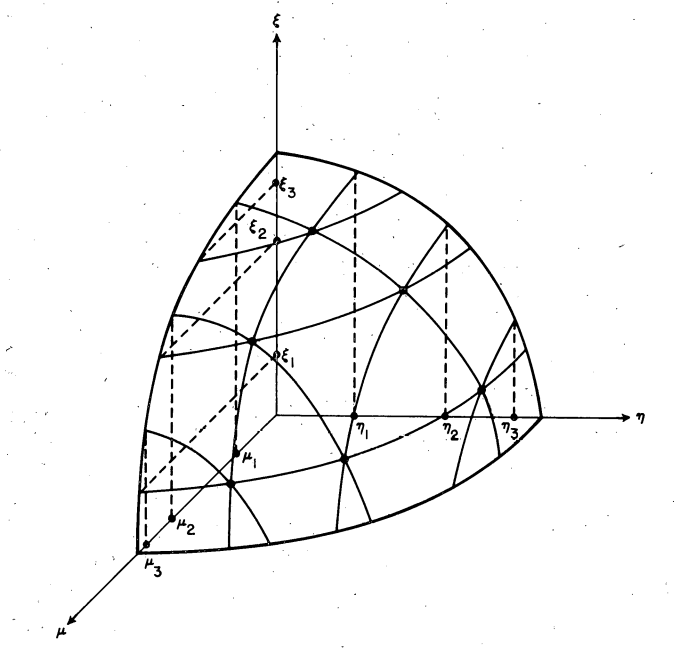
\includegraphics[scale=0.5]{./images/quadrature_octant.png} 
	\caption{One octant of a $S_6$ 3D quadrature set. $N=6$ because there are 6 angular points on each axis in the positive and negative directions~\cite{Lathrop}} 
	\label{fig:3D_quad}
\end{figure}

\section{Discretising the transport equation}

The S$_N$ method is essentially the approach one reaches if we discretise all variables in the traditional fashion in numerical methods:
\begin{itemize}
	\item Energy is discretised by the multi-group method as usual
	\item Angle is discretised by the discrete ordinates approximation
	\item Space is discretised by the finite difference method (or finite element method)
\end{itemize}
We have already seen finite difference discretisation in the diffusion coursework. Now we apply it to a slightly different differential equation, the 1D version of Eq.~\eqref{eq:transport_DO}:
\begin{equation}\label{eq:DO}
	 \left[\mu_n\frac{\partial}{\partial x} + \Sigma_\mathrm{t}\right]\psi_n
	= Q\;\mathrm{,}
\end{equation}
where $\psi_n = \psi(x,\mu_n)$, with $\mu_n$ the cosine that the (discretised) neutron flight direction makes with the $x$ axis, and where $Q$ is given by:
\begin{equation}
	Q = \frac{1}{2k}\nu\Sigma_\mathrm{f}\phi + \frac{1}{2}\Sigma_\mathrm{s}\phi\;\mathrm{.}
\end{equation}

The spatial discretisation of the domain proceeds as before: we divide the spatial domain into $I$ intervals as in Fig.~\ref{fig6}:
\begin{figure}[hb]
    \centering
    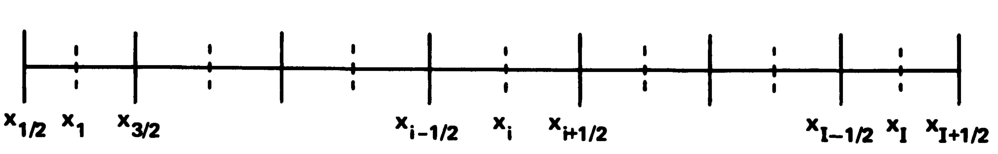
\includegraphics[width=0.6\linewidth]{images/fig6.png}
    \caption{Spatial mesh for computation~\cite{Lewis}}
    \label{fig6}
\end{figure}
The $i$-th interval in the spatial mesh has a left boundary at $x_{i-1/2}$, a midpoint $x_i$, and a right boundary $x_{i+1/2}$; the width is therefore $\Delta x_i=x_{i+1/2}-x_{i-1/2}$. The angular flux value at the left boundary $x_{i-1/2}$ is denoted as $\psi_{n,i-1/2}=\psi(x_{i-1/2},\mu_n)$; and the angular flux values at the right boundary $x_{i+1/2}$ is accordingly $\psi_{n,i+1/2}$. Within each interval, the cross sections are assumed to have constant values $\Sigma_{t,i}$.

We relate all these quantities together by integrating Eq.~\eqref{eq:DO} over the $i$-th interval:
\begin{align}
    \mu_n\int_{x_{i-1/2}}^{x_{i+1/2}}\frac{\partial\psi_n}{\partial x}\,dx+\int_{x_{i-1/2}}^{x_{i+1/2}}\Sigma_t(x)\psi_n(x)\,dx&=\int_{x_{i-1/2}}^{x_{i+1/2}}Q(x)\,dx \\
    \Longrightarrow\quad\mu_n\left(\psi_{n,i+1/2}-\psi_{n,i-1/2}\right)+\Sigma_{t,i}\int_{x_{i-1/2}}^{x_{i+1/2}}\psi_n(x)\,dx&=\int_{x_{i-1/2}}^{x_{i+1/2}}Q(x)\,dx
\end{align}
If we define the mesh-averaged flux $\psi_{n,i}$ and mesh-averaged source\footnote{The subscript $n$ is redundant for our isotropic source but we keep it for a more consistent notation.} $Q_{n,i}$ as:
\begin{equation}\label{SN12}
    \psi_{n,i}=\frac{1}{\Delta x_i}\int_{x_{i-1/2}}^{x_{i+1/2}}\psi_n(x)\,dx,\quad Q_{n,i}=\frac{1}{\Delta x_i}\int_{x_{i-1/2}}^{x_{i+1/2}}Q(x)\,dx
\end{equation}
then we have our \textit{difference equation} as follows:
\begin{equation}\label{SN5}
    \mu_n\left(\psi_{n,i+1/2}-\psi_{n,i-1/2}\right)+\Sigma_{t,i}\Delta x_i\psi_{n,i}=\Delta x_i Q_{n,i}
\end{equation}
At this point, we know the quantities $\mu_n,\,\Sigma_{t,i}$ and $\Delta x_i$. Moreover, since the source term $Q(x)$ is known, we can calculate $Q_{n,i}$ so that it is also a known quantity. For an imposed boundary condition (for example, for $\mu_n>0$ the flux value of $\psi_{n,i-1/2}$ will be imposed), we have two unknowns: (1) the mesh-averaged flux $\psi_{n,i}$ which we can use to calculate the scalar flux and (2) the flux value at the other boundary ($\psi_{n,i+1/2}$ in our example). To close the system, we will require an additional \textit{closure relation} to eliminate one of the unknowns. These describe how the angular flux changes across a mesh.

\subsection{Closure relations}
\subsubsection{Diamond-differencing}
The \textit{diamond-differencing} closure assumes that $\psi_n(x)$ varies linearly within the interval, so that:
\begin{equation}\label{SN5DD}
    \psi_{n,i}=\frac{1}{2}\left(\psi_{n,i-1/2}+\psi_{n,i+1/2}\right)
\end{equation}
Applying the diamond-differencing closure to Eq.~\eqref{SN5} gives:
\begin{align}
    &\text{if }\mu_n>0\text{, then }\psi_{n,i}=\frac{\Delta x_iQ_{n,i}+2|\mu_n|\psi_{n,i-1/2}}{\Delta x_i\Sigma_{t,i}+2|\mu_n|}\quad\text{with } \psi_{n,i+1/2}=2\psi_{n,i}-\psi_{n,i-1/2}\label{SN5DDr}\\
    &\text{if }\mu_n<0\text{, then }\psi_{n,i}=\frac{\Delta x_iQ_{n,i}+2|\mu_n|\psi_{n,i+1/2}}{\Delta x_i\Sigma_{t,i}+2|\mu_n|}\quad\text{with }\psi_{n,i-1/2}=2\psi_{n,i}-\psi_{n,i+1/2}\label{SN5DDl}
\end{align}
This method is \textit{second-order accurate} in space (meaning a coarser spatial discretisation can be used) but can lead to negative fluxes when meshes are optically thick which can cause numerical problems.

\subsubsection{Step method}
The \textit{step method} closure is defined as:
\begin{align}
    &\text{if }\mu_n>0\text{, then }\psi_{n,i+1/2}=\psi_{n,i}\\
    &\text{if }\mu_n<0\text{, then }\psi_{n,i-1/2}=\psi_{n,i}
\end{align}
Applying the step method closure to Eq.~\eqref{SN5} gives:
\begin{align}
    &\text{if }\mu_n>0\text{, then }\psi_{n,i}=\frac{\Delta x_iQ_{n,i}+|\mu_n|\psi_{n,i-1/2}}{\Delta x_i\Sigma_{t,i}+|\mu_n|}\quad\text{with } \psi_{n,i+1/2}=\psi_{n,i}\label{SN5SMr}\\
    &\text{if }\mu_n<0\text{, then }\psi_{n,i}=\frac{\Delta x_iQ_{n,i}+|\mu_n|\psi_{n,i+1/2}}{\Delta x_i\Sigma_{t,i}+|\mu_n|}\quad\text{with }\psi_{n,i-1/2}=\psi_{n,i}\label{SN5SMl}
\end{align}
While this is only first-order accurate in space, it guarantees fluxes remain positive.

\subsection{Transport sweeps}

Putting the difference equation, Eq.~\eqref{SN5}, and one of the several closure relations together, we can obtain a relationship between the incoming and outgoing angular fluxes in a mesh cell:
\begin{align}
    &\text{if }\mu_n>0\text{, then }\psi_{n,i+1/2}=\mathcal{A}_{n,i}\psi_{n,i-1/2}+\mathcal{B}_{n,i}Q_{n,i}\label{SN5r}\\
    &\text{if }\mu_n<0\text{, then }\psi_{n,i-1/2}=\mathcal{C}_{n,i}\psi_{n,i+1/2}+\mathcal{D}_{n,i}Q_{n,i}\label{SN5l}
\end{align}
Here $\mathcal{A}_{n,i}$, $\mathcal{B}_{n,i}$, $\mathcal{C}_{n,i}$, and $\mathcal{D}_{n,i}$ are simply scalars which vary depending on the closure relation chosen. The $\mu_n>0$ and $\mu_n<0$ directions are considered separately to construct marching schemes that follow the direction of travelling neutrons. Suppose we know the incoming flux distribution on the leftmost boundary $x_{1/2}$; this specifies $\psi_{n,1/2}$ for $\mu_n>0$ directions. We can then solve for $\psi_{n,3/2},\psi_{n,5/2},\dots$ with Eq.~\eqref{SN5r} sweeping rightwards. Likewise, the incoming flux on the rightmost boundary specifies $\psi_{n,I+1/2}$ for $\mu_n<0$ directions and we solve $\psi_{n,I-1/2},\psi_{n,I-3/2},\dots$ using Eq.~\eqref{SN5l} sweeping leftwards. The required incoming flux distributions are the \textit{boundary conditions} to the closed system of equations.
\subsubsection{Tallying across sweeps}
We are usually only interested in angle-integrated quantities such as scalar flux $\phi(x)$ defined by:
\begin{equation}
    \phi(x)=\sum_{n=1}^N w_n\,\psi_n(x)
\end{equation}
The mesh-averaged scalar flux is thus:
\begin{equation} \label{SN14}
    \phi_i=\frac{1}{\Delta x_i}\int_{x_{i-1/2}}^{x_{i+1/2}}\phi(x)\,dx=\sum_{n=1}^N w_n\,\psi_{n,i}
\end{equation}
This suggests a convenient feature of transport sweeps: \textbf{after calculating} $\psi_{n,i}$ \textbf{at each marching step in the sweep we can tally the contribution} $w_n\,\psi_{n}$ \textbf{to the scalar flux} $\phi_i$ \textbf{after which we can discard the value of} $\psi_{n,i}$. \textbf{Thus we only track} $I$ \textbf{values of} $\phi_{n,i}$, \textbf{and we do not need to track all} $(N\times I)$ \textbf{values of} $\psi_{n,i}$ \textbf{across sweeps}.

This provides a substantial saving in memory which would not be possible if we had to construct a matrix relating all values of $\psi_{n,i}$ to each other.

When going to 2D or 3D, the nature of the transport sweep remains nearly exactly the same. The main difference is that instead of starting from the left or right, one starts from the 4 corners of a square (in 2D) or the 8 corners of a cube (in 3D) and the problem is solved as a \textbf{wave front} moving from one side of the problem to the other.

\subsection{Boundary conditions}
We saw that the complete specification of the closed system of equations required a set of boundary conditions be specified. We consider here three common sets of boundary conditions: \textit{vacuum}, \textit{periodic}, and \textit{reflective}. 

For periodic and reflective conditions, some particularly clever means of solving these problems are presented here. However, most codes tend to simply guess some value of the boundary angular flux and then iterate the sweep until its value stops changing substantially.

\subsubsection{Vacuum boundary conditions}
The vacuum boundary conditions apply when there are no incoming neutrons into the domain, such that:
\begin{align}
    &\text{if }\mu_n>0\text{, then }\psi_{n,1/2}=0\\
    &\text{if }\mu_n<0\text{, then }\psi_{n,I+1/2}=0
\end{align}
Solving the closed system of equations for vacuum boundary conditions is straightforward; set the appropriate boundary values to zero and sweep accordingly.
\subsubsection{Periodic boundary conditions}
The periodic boundary conditions consider the domain to be one element in an infinitely repeating lattice. In such a lattice, the outgoing flux distribution of neutrons leaving at one boundary is matched by the incoming flux distribution of neutrons entering at the other boundary, such that:
\begin{equation}\label{SN7}
    \text{for any }\mu_n\text{, then }\psi_{n,1/2}=\psi_{n,I+1/2}
\end{equation}
We consider Eq.~\eqref{SN5r} for the $\mu_n>0$ direction, and write out explicitly what happens in a full sweep. We have:
\begin{align}
    \psi_{n,I+1/2}&=\mathcal{A}_{n,I}\psi_{n,I-1/2}+\mathcal{B}_{n,I}Q_{n,I}\\
    &=\mathcal{A}_{n,I}\mathcal{A}_{n,I-1}\psi_{n,I-3/2}+\mathcal{A}_{n,I}\mathcal{B}_{n,-1I}Q_{n,I-1}+\mathcal{B}_{n,I}Q_{n,I} \\
    &=\dots \nonumber \\
    &=\left(\prod_{i=1}^I\mathcal{A}_{n,i}\right)\psi_{n,1/2}+
    \begin{bmatrix}
        \text{terms that do not} \\
        \text{ depend on boundary conditions }
    \end{bmatrix} \label{SN6}
\end{align}
In particular, if we used a vacuum boundary condition that $\psi^\text{vac}_{n,1/2}=0$ it follows from Eq.~\eqref{SN6} that:
\begin{equation}
    \psi^\text{vac}_{n,I+1/2}=
    \begin{bmatrix}
        \text{terms that do not} \\
        \text{ depend on boundary conditions }
    \end{bmatrix}
\end{equation}
which can be inserted back into Eq.~\eqref{SN6} to give:
\begin{equation}
    \psi_{n,I+1/2}=\left(\prod_{i=1}^I\mathcal{A}_{n,i}\right)\psi_{n,1/2}+\psi^\text{vac}_{n,I+1/2}
\end{equation}
Now, if we impose the periodic boundary condition of Eq.~\ref{SN7} we have:
\begin{equation}
    \psi_{n,1/2}=\psi_{n,I+1/2}=\psi^\text{vac}_{n,I+1/2}\bigg/\left[1-\prod_{i=1}^I\mathcal{A}_{n,i}\right]
\end{equation}
Thus we see that solving the closed system of equations for periodic boundary conditions requires:
\begin{enumerate}
    \item First we solve once with vacuum boundary conditions $\psi^\text{vac}_{n,1/2}=0$ to obtain $\psi^\text{vac}_{n,I+1/2}$ and tally $\prod\mathcal{A}_{n,i}$;
    \item Then we calculate the periodic boundary fluxes $\psi_{n,I+1/2}$ for a final sweep.
\end{enumerate}
The case for the $\mu_n>0$ direction follows analogously.
\subsubsection{Reflective boundary conditions}
The reflective boundary conditions consider neutrons to undergo specular reflection at the boundaries. If we introduce the notation:
\begin{align*}
    \overrightarrow{\psi}_{n,1/2}=\psi(x_{1/2},\mu_n)&,\quad
    \overleftarrow{\psi}_{n,1/2}=\psi(x_{1/2},-\mu_n) \\
    \overrightarrow{\psi}_{n,I+1/2}=\psi(x_{I+1/2},\mu_n)&,\quad
    \overleftarrow{\psi}_{n,I+1/2}=\psi(x_{I+1/2},-\mu_n)
\end{align*}
then reflective boundary conditions are such that:
\begin{align}
    \overrightarrow{\psi}_{n,1/2}&=\overleftarrow{\psi}_{n,1/2}\quad\text{and} \label{SN8l} \\
    \overrightarrow{\psi}_{n,I+1/2}&=\overleftarrow{\psi}_{n,I+1/2} \label{SN8r}
\end{align}
We carry out an analysis similar to the previous section. We start at the left boundary and sweep in the $\mu_n>0$ direction to obtain:
\begin{equation}
    \overrightarrow{\psi}_{n,I+1/2}=\left(\prod_{i=1}^I\mathcal{A}_{n,i}\right)\overrightarrow{\psi}_{n,1/2}+
    \begin{bmatrix}
        \text{terms that do not} \\
        \text{ depend on boundary conditions }
    \end{bmatrix}
\end{equation}
By Eq.~\eqref{SN8r} this is equal to $\overleftarrow{\psi}_{n,I+1/2}$, which we use to sweep in the $\mu_n<0$ direction to obtain:
\begin{align}
    \overleftarrow{\psi}_{n,1/2}&=\left(\prod_{i=1}^I\mathcal{C}_{n,i}\right)\overrightarrow{\psi}_{n,I+1/2}+
    \begin{bmatrix}
        \text{even more terms that do not} \\
        \text{ depend on boundary conditions }
    \end{bmatrix} \\
    &=\left(\prod_{i=1}^I\mathcal{C}_{n,i}\right)\left(\prod_{i=1}^I\mathcal{A}_{n,i}\right)\overrightarrow{\psi}_{n,1/2}+
    \begin{bmatrix}
        \text{all the terms that do not} \\
        \text{ depend on boundary conditions }
    \end{bmatrix}
\end{align}
If we used a vacuum boundary condition that $\overrightarrow{\psi}^\text{vac}_{n,1/2}=0$ to calculate $\overleftarrow{\psi}^\text{vac}_{n,1/2}$, then we will have:
\begin{equation}
    \overleftarrow{\psi}_{n,1/2}=\left(\prod_{i=1}^I\mathcal{C}_{n,i}\right)\left(\prod_{i=1}^I\mathcal{A}_{n,i}\right)\overrightarrow{\psi}_{n,1/2}+\overleftarrow{\psi}^\text{vac}_{n,1/2}
\end{equation}
so that imposing the reflective boundary condition of Equation \ref{SN8l} gives:
\begin{equation}
    \overrightarrow{\psi}_{n,1/2}=\overleftarrow{\psi}_{n,1/2}=\overleftarrow{\psi}^\text{vac}_{n,1/2}\bigg/\left[1-\left(\prod_{i=1}^I\mathcal{C}_{n,i}\right)\left(\prod_{i=1}^I\mathcal{A}_{n,i}\right)\right]
\end{equation}
Thus we see that solving the closed system of equations for periodic boundary conditions requires:
\begin{enumerate}
    \item First we start at the left boundary with vacuum boundary conditions $\overrightarrow{\psi}^\text{vac}_{n,1/2}=0$ and sweep right to obtain $\overrightarrow{\psi}^\text{vac}_{n,I+1/2}$ and tally $\prod\mathcal{A}_{n,i}$;
    \item Second we set $\overleftarrow{\psi}_{n,I+1/2}=\overrightarrow{\psi}^\text{vac}_{n,I+1/2}$ at the right boundary and sweep left to obtain $\overleftarrow{\psi}^\text{vac}_{n,1/2}$ and tally $\prod\mathcal{C}_{n,i}$;
    \item Then we calculate the reflective boundary fluxes $\overrightarrow{\psi}_{n,1/2}$ for a final sweep.
\end{enumerate}
The case for the right boundary follows analogously.

\section{Source/power iteration with transport solvers}

All of the discussion so far has focused on solving Eq.~\eqref{eq:DO}, i.e.,
\begin{equation*}
	 \left[\mu_n\frac{\partial}{\partial x} + \Sigma_\mathrm{t}\right]\psi_n
	= Q\;\mathrm{,}
\end{equation*}
for a fixed isotropic source, $Q$. Unless the medium is purely absorbing, $Q$ is not fixed: it will either change due to the scattering source (in non-fissile problems) or the scattering and fission sources (in fissile problems). These must be updated once a transport sweep is complete. 

In principle, for eigenvalue problems, scattering and fission sources could be updated separately. This would mean having \textbf{two} loops: an inner iteration (known as source iteration) where the scattering source is updated, and an outer iteration (known as power iteration) where the fission source is updated. Alternatively, both sources may be updated at the same time -- but this can have implications for the speed of convergence.

Here we will update both sources at once. As a result, the $k$-eigenvalue algorithm for $S_N$ looks very much like the algorithm for diffusion:
\begin{enumerate}
    \item Begin with an initial guess for the scalar flux vector $\phi_i$ and eigenvalue $k$. Suppose we set everything to 1:
    \begin{equation}
        \phi^{(0)}_i=[1,1,\dots],\quad k^{(0)}=1
    \end{equation}
    \item Compute the source vector for the next iteration with:
    \begin{equation}
        Q^{(j+1)}_{n,i}=\frac{1}{2}\left(\Sigma_{s,i}+\frac{1}{k^{(j)}}\bar{\nu}\Sigma_{f,i}\right)\phi^{(j)}_i
    \end{equation}
    and initialise an empty scalar flux vector $\phi^{(j+1)}_i=[0,0,\dots]$.
    \item For each abscissa $\mu_n$, perform the required sweeps in accordance with the chosen closure and imposed boundary conditions to converge each $\psi^{(j+1)}_{n,i}$. Perform one last sweep with the converged $\psi^{(j+1)}_{n,i}$; at each marching step in the sweep we compute and add onto the new scalar flux vector the contribution:
    \begin{equation}
        \phi^{(j+1)}_i\rightarrow\phi^{(j+1)}_i + w_n\,\psi_{n,i}
    \end{equation}
    \item We update the eigenvalue :
    \begin{equation}
        k^{(j+1)}=k^{(j)}\left[\sum_{i=1}^I\Delta x_i\cdot\bar{\nu}\Sigma_{f,i}\cdot\phi^{(j+1)}_i\right]
        \bigg/\left[\sum_{i=1}^I\Delta x_i\cdot\bar{\nu}\Sigma_{f,i}\cdot\phi^{(j)}_i\right]
    \end{equation}
    \item Update the iteration index and iterate Steps 2-4 until the scalar flux and eigenvalue have converged within specified tolerances:
    \begin{equation}
        \max_i\left(\frac{|\phi^{(j+1)}_i-\phi^{(j)}_i|}{|\phi^{(j)}_i|}\right)<\varepsilon_1,\quad\text{and}\quad\frac{|k^{(j+1)}-k^{(j)}|}{|k^{(j)}|}<\varepsilon_2
    \end{equation}
\end{enumerate}

\section{Practicalities of the $S_N$ method}

For many years, $S_N$ has been the work-horse transport method in many areas, especially national security. This is because it is fast, low memory, relatively easy to understand and implement, and works in `general' geometries. However, there are several substantial drawbacks to the method which occur in more complicated problems.

\subsection{Geometric limitations}

The sweeping procedure described before is fast and can be applied, in principle, to a wide variety of unstructured meshes in 3D. However, the method relies on a mesh element being intersected once and only once for a given sweep direction. This causes problems if, say, we have curved geometries (such as in nuclear reactors). The result is that S$_N$ solvers require either `rectangularlised'/`triangularised' meshes (which risks losing accuracy) or a very fine mesh discretisation to try to preserve curved features of the geometry. This is a significant reason why MoC (which can use curved geometries) is used much more frequently than S$_N$ for nuclear reactor calculations. On the other hand, S$_N$ uses less memory than (standard) MoC due to MoC's need to perform ray tracing and remember the track lengths across the problem.

\subsection{Negative fluxes}

As mentioned earlier, the popular diamond differencing scheme is fast and accurate, but can result in negative fluxes when spatial discretisation is not sufficiently fine. This is very concerning because negative fluxes are non-physical. Even worse, this can cause simulations to fail entirely. 

Fortunately, several possible remedies exist. One solution to this may be to more finely discretise a problem where this occurs, but that can become prohibitively expensive. Similarly, one can use the characteristic closure which ensure positivity of fluxes -- but this is also more expensive. Ultimately, what many codes do is `live with it' by checking, every iteration, during the sweep, whether negative scalar fluxes have occurred and then setting them to 0 with some rebalance of fluxes to ensure particle conservation. This approach is referred to as `flux fix-up' and may slow down the convergence of simulations, but it is often survivable.

As an aside, MoC can also use different closures in principle! This has been investigated and shown to have some benefits. It can also suffer from negative fluxes if using diamond differencing.

\subsection{The ray effect}

In 2D or 3D problems with relatively little scattering and localised neutron sources (such as shielding problems), it is possible to obtain a numerical artefact known as the ray effect. Essentially this is a non-physical imprint of the quadrature on the simulation, e.g., a star shape about a fixed source in the centre of a problem. This is because the sparse quadrature is ineffective at interpolating the fluxes between quadrature directions.

An illustration of the ray effect is given for a purely absorbing problem with a small source in the centre in Fig.~\ref{fig:ray_effect}. The quadrature uses 8 points in the azimuthal direction. Naturally, the correct solution should be azimuthally uniform.

There are several algorithmic tricks which attempt to remedy the ray effect, but the most reliable is to simply increase the order of the quadrature, at the cost of greater computational expense.

This can also affect MoC. However, ray effect is much less severe in LWR problems as neutron sources are distributed throughout the geometry and fluxes tend (over reasonably large volumes) to be closer to isotropic.

\begin{figure}[h!]
	\centering
	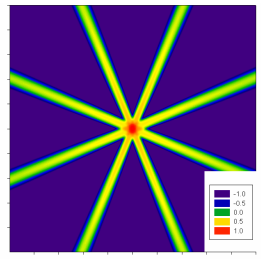
\includegraphics{./images/ray_effect.png} 
	\caption{Ray effect demonstration showing the logarithm of the scalar flux~\cite{Stone2007}} 
	\label{fig:ray_effect}
\end{figure}

\printbibliography

\end{document}
